\chapter{PAG 6.1}
\section{Aim}
To complete a multi-stage process for the synthesis, purification, and identification of aspirin
\section{Research}
In PAG 6.1, students carry out the synthesis of aspirin, an organic solid, using a two-stage process starting from the oil of wintergreen. 
In the first stage, the oil of wintergreen, which contains methyl 2-hydroxybenzoate, is hydrolysed by heating under reflux with sodium hydroxide solution to produce 2-hydroxybenzoic acid (salicylic acid).
\\\\
\noindent
In the second stage, the 2-hydroxybenzoic acid is esterified using ethanoic anhydride to form aspirin (2-ethanoyloxybenzoic acid, or acetylsalicylic acid). The aspirin is recrystallised and analysed by thin layer chromatography and by melting temperature.
\\\\
\begin{figure}[htp]
 \centering
 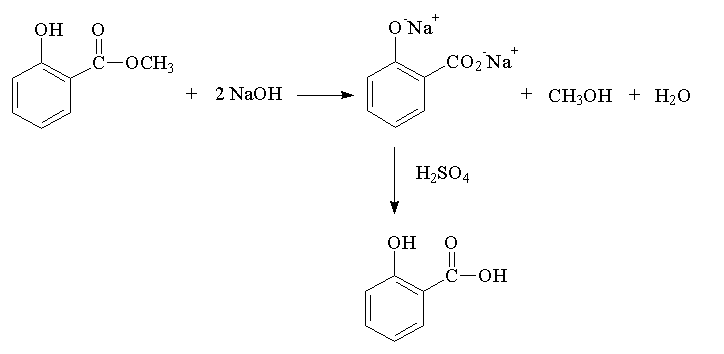
\includegraphics[scale=0.35]{salicylic-acid-syn.png}
 \caption{Production of Salicylic Acid \cite{olmsted1998synthesis}}
\end{figure}
\newpage
\noindent
The above reaction shows the production of Salicylic Acid from Oil of Wintergreen. It uses NaOH and \ce{H2SO4} to produce 2-hydroxybenzoic Acid.

\begin{figure}[htp]
 \centering
 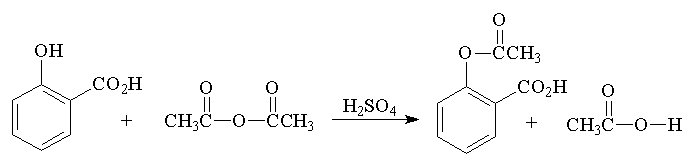
\includegraphics[scale=0.5]{aspirin actual.png}
 \caption{Production of Aspirin \cite{raubenheimer1913chemistry}}
\end{figure}
\noindent
Figure 1.2 shows the production of Aspirin from Salicylic Acid. 

\section{Specification Point}
\textbf{Techniques and procedures:}
\begin{itemize}
    \item The synthesis and purification of a solid organic compound e.g. Aspirin 
    \item The technique of thin layer chromatography (TLC), location of spots and interpretation
    \item Melting point determination
    \item Filtration and Recrystallisation
\end{itemize}


\chapter{Prep of Salicylic Acid}
\section{Equipment}
\begin{small}
\begin{multicols}{2}
\begin{itemize}
    \item Eye Protection
    \item Mass balance
    \item Measuring Cylinder (10\si{\centi\meter\cubed})
    \item Measuring Cylinder (50\si{\centi\meter\cubed})
    \item Quick-fit apparatus
    \item Pear-shaped flask (50\si{\centi\meter\cubed})
    \item Liebig condenser and tubing
    \item Retort stand, boss and clamp
\end{itemize}
\columnbreak
\begin{itemize}
    \item Anti-bumping granules
    \item Water bath
    \item Beaker (100\si{\centi\meter\cubed})
    \item Ice Bucket
    \item Distilled Water
    \item Dropping pipette
    \item Stirring rod
    \item Filtration apparatus
    \item Watch glass
\end{itemize}
\end{multicols}
\end{small}


\section{Risk Assessment}
\begin{center}
\begin{tabularx}{0.8\textwidth} { 
  | >{\raggedright\arraybackslash}X 
  | >{\raggedright\arraybackslash}X 
  | >{\raggedright\arraybackslash}X | }
 \hline
 \textbf{Identity} & \textbf{Hazard Info} & \textbf{Prevention} \\
 \hline
 2.0 \si[per-mode=symbol]{\mol\per\dm\cubed} NaOH(aq)  & Danger to skin and eyes. Harmful if swallowed  & Wear splashproof goggles. Avoid inhalation and take care when transferring NaOH  \\
 \hline
\end{tabularx}
\end{center}
\newpage
\begin{center}
\begin{tabularx}{0.8\textwidth} { 
  | >{\raggedright\arraybackslash}X 
  | >{\raggedright\arraybackslash}X 
  | >{\raggedright\arraybackslash}X | }
 \hline
 2.0 \si[per-mode=symbol]{\mol\per\dm\cubed} HCl(aq)  & Danger to skin and eyes. Harmful if swallowed  & Wear splashproof goggles. \\
 \hline
 Oil of Wintergreen & Can cause eye irritation and harmful if swallowed. & Keep lab well ventilated and wear eye protection \\
 \hline
\end{tabularx}
\end{center}
\section{Method}
\begin{enumerate}
\item Set up the apparatus for reflux using a 50\si{\centi\meter\cubed} pear-shaped flask and Liebig condenser.
\item Add about 2.5 cm3 oil of wintergreen to a 10\si{\centi\meter\cubed} measuring cylinder and record the mass.
\item Pour the oil of wintergreen into the pear-shaped flask.
\item Record the mass of the measuring cylinder again.
\item Using a 50\si{\centi\meter\cubed} measuring cylinder, measure about 25\si{\centi\meter\cubed} of 2.0 \si[per-mode=symbol]{\mol\per\dm\cubed} sodium hydroxide solution.
\item Add the sodium hydroxide solution to the pear-shaped flask. Add a few anti-bumping granules.
\item Heat the reaction mixture under reflux using a boiling water bath, sand bath or electric heater, for about 30 minutes.
\item Leave the mixture to cool, then pour into a 50\si{\centi\meter\cubed} beaker which is being cooled in a larger beaker of ice and water. 
\item Neutralise the reaction mixture by carefully add 2.0 \si[per-mode=symbol]{\mol\per\dm\cubed} hydrochloric acid to the mixture dropwise, stirring with a stirring rod. Keep adding acid until no more solid forms.
\item Filter the solid product from the reaction mixture using filtration under reduced pressure and wash with a small amount of cold distilled water.
\item Measure and record the mass of a watchglass, then transfer the solid product to the watchglass and leave to dry.
\item When the solid is dry, record the mass of the solid and the watchglass.
\item Store the product in a labelled, clean, dry sample tube for use in Part 2. 
\end{enumerate}

\section{Results Table}
\begin{center}
\begin{tabularx}{0.8\textwidth} { 
  | >{\raggedright\arraybackslash}X
  | >{\raggedright\arraybackslash}X
  | >{\raggedright\arraybackslash}X | }
 \hline
 Mass of Cylinder/g & Mass of Wintergreen/g & Mass of Salicylic Acid \\
 \hline
 35.54 & 7.52 & \\
\hline
\end{tabularx}
\end{center}
\chapter{Prep of Aspirin}
\section{Equipment}
\begin{small}
\begin{multicols}{2}
\begin{itemize}
    \item Splashproof goggles
    \item Mass Balance
    \item Distilled water
    \item Clean and dry sample tube with lid
    \item Conical flask (100\si{\centi\meter\cubed})
    \item 2 x Measuring cylinders (10\si{\centi\meter\cubed})
    \item Spatula 
\end{itemize}
\columnbreak
\begin{itemize}
    \item Stirring rod
    \item Ice bucket
    \item Filtration Apparatus
    \item Watch Glass
    \item Sample tube and lid
    \item Glass marker pen
\end{itemize}
\end{multicols}
\end{small} 

\section{Risk Assessment}
\begin{center}
\begin{tabularx}{0.8\textwidth} { 
  | >{\raggedright\arraybackslash}X 
  | >{\raggedright\arraybackslash}X 
  | >{\raggedright\arraybackslash}X | }
 \hline
 \textbf{Identity} & \textbf{Hazard Info} & \textbf{Prevention} \\
 \hline
 Ethanoic Anhydride (\ce{CH3CO)2O}) & Danger to skin and eyes. & Store safely, maintain hygeine before, during and after use. \\
 \hline
 Concentrated \ce{H2SO4} & Can cause severe skin burns and eye damage. & Wear eye protection and gloves. \\
 \hline
 Concentrated Ethanoic Acid (\ce{CH3CO2H}) & Can cause severe skin and eye damage. Releases flammable vapours & Wear eye protection, gloves and avoid inhalation. \\
 \hline
 \end{tabularx}
\end{center}
\newpage
\section{Method}
\begin{enumerate}
    \item Transfer about 2 g of the 2-hydroxybenzoic acid you made in Part 1 into the sample tube. Measure and record the mass of the sample tube and sample.
    \item Transfer the 2-hydroxybenzoic acid into a 100\si{\centi\meter\cubed} conical flask and measure the mass of the sample tube again. 
    \item Measure 4\si{\centi\meter\cubed} ethanoic anhydride into a 10\si{\centi\meter\cubed} dry measuring cylinder, and pour into the conical flask.
    \item Add five drops of concentrated sulfuric(VI) acid to the flask and shake gently from side to side for about 10 minutes.
    \item Cool the conical flask in a large beaker containing crushed ice to complete the crystallisation.
    \item Using a clean measuring cylinder, measure 4\si{\centi\meter\cubed} of cold glacial ethanoic acid and add this to the reaction mixture to dilute it.
    \item Filter off the solid product using filtration under reduced pressure, washing once with ice-cold distilled water.
    \item Measure and record the mass of a watchglass and then transfer the solid product to the watchglass and leave to dry.
    \item When the solid is dry, record the mass of the solid and the watchglass.
    \item Store the product in a labelled, clean, dry sample tube for recrystallisation in Part 3. 
\end{enumerate}

\section{Results Table}
\begin{center}
\begin{tabularx}{0.8\textwidth} { 
  | >{\raggedright\arraybackslash}X
  | >{\raggedright\arraybackslash}X
  | >{\raggedright\arraybackslash}X | }
 \hline
 Mass of Sample tube and Sample/g & Mass of sample/g & Mass of Solid/g \\
 \hline
 ㅤ&ㅤ&ㅤ& \\
 \hline
\end{tabularx}
\end{center}
\newpage
\chapter{Recrystallisation}
\section{Equipment}
\begin{small}
\begin{multicols}{2}
\begin{itemize}
    \item Eye Protection
    \item Mass Balance
    \item 2 x Conical Flask 100\si{\centi\meter\cubed}
    \item Dropping Pipette
    \item Spatula
    \item Stirring Rod
\end{itemize}
\columnbreak
\begin{itemize}
    \item Large Beaker
    \item Water Bath
    \item Filtration Apparatus
    \item Watchglass
    \item Sample tube and lid
    \item Glass marker pen
\end{itemize}
\end{multicols}
\end{small}

\section{Risk Assessment}
\begin{center}
\begin{tabularx}{0.8\textwidth} { 
  | >{\raggedright\arraybackslash}X 
  | >{\raggedright\arraybackslash}X 
  | >{\raggedright\arraybackslash}X | }
 \hline
 \textbf{Identity} & \textbf{Hazard Info} & \textbf{Prevention} \\
 \hline
 Ethanol \ce{C2H5OH} & Highly flammable liquid. & Store safely, keep away from flames \\
 \hline
 \end{tabularx}
\end{center}
\section{Method}
\begin{enumerate}
    \item Transfer the majority of you impure aspirin to a 100\si{\centi\meter\cubed} conical flask. Save a few crystals for analysis by chromatography in Part 4.
    \newpage
    \item Warm approximately 30 cm3 of ethanol in another 100\si{\centi\meter\cubed} conical flask, using an electric water bath/heating mantle/sand bath. 
    \item Add small amounts (0.5\si{\centi\meter\cubed}) of hot ethanol at a time to the impure aspirin until it has all just dissolved. 
    \item Quickly filter the hot solution using reduced pressure filtration, washing with a minimal small amount of hot ethanol. 
    \item Cool the filtrate slowly until needle-like crystals of aspirin form, then in an ice–water bath.
    \item Filter the aspirin crystals, again using reduced pressure filtration and wash with ice-cold ethanol.
    \item Measure and record the mass of a watchglass, then transfer the recrystallised aspirin to the watchglass and leave to dry.
    \item When the solid is dry, measure and record the mass of the solid and the watchglass.
    \item Transfer the aspirin into a labelled, clean, dry sample tube.
\end{enumerate}

\section{Results Table}
\begin{center}
\begin{tabularx}{0.8\textwidth} { 
  | >{\raggedright\arraybackslash}X
  | >{\raggedright\arraybackslash}X | }
 \hline
 Mass of Watchglass + Aspirin/g & Mass of Aspirin/g  \\
 \hline
 ㅤ&ㅤ&ㅤ& \\
\hline
\end{tabularx}
\end{center}
\chapter{Chromatography}
\section{Equipment}
\begin{small}
\begin{itemize}
    \item Eye Protection
    \item UV Light
    \item 5 Watchglasses
    \item Dropping Pipette
    \item Thin layer chromatography plate
    \item Beaker 100\si{\centi\meter\cubed}
    \item Watchglass
    \item Pencil
\end{itemize}
\end{small}

\section{Risk Assessment}
\begin{center}
\begin{tabularx}{0.8\textwidth} { 
  | >{\raggedright\arraybackslash}X 
  | >{\raggedright\arraybackslash}X 
  | >{\raggedright\arraybackslash}X | }
 \hline
 \textbf{Identity} & \textbf{Hazard Info} & \textbf{Prevention} \\
 \hline
 Aspirin & Can cause skin irritation and respiratory problems & Store safely, avoid inhalation \\
 \hline
 Ethanol \ce{C2H5OH} & Highly flammable liquid. & Store safely, keep away from flames. \\
 \hline
 Iodine Crystals (\ce{I2}) & Toxic, can cause respiratory problems & Store safely avoid inhalation \\
 \hline
 Salicylic Acid & Contact with skin can cause irritation & Avoid contact with skin \\
 \hline
 \end{tabularx}
 \end{center}
\section{Method}
\begin{enumerate}
    \item Prepare your thin layer chromatography (TLC) plate by drawing a line in pencil about 1 cm from the bottom. Mark four crosses along the line. These crosses are where the samples will be placed. 
    \item Pour a 5mm depth of chromatography solvent into a 100 cm3 beaker and cover the beaker with a watchglass. 
    \item Place 2-3 crystals of the pure aspirin sample on a watchglass and dissolve in a drop of ethanol.
    \item Place the capillary/pipette in the solution to draw up a small amount, then briefly touch to the first cross to apply the solution to the TLC plate. Alternatively, use a fine artist paint brush.
    \item Allow the spot to dry, then repeat 3-4 more times, ensuring that the final diameter is no greater than 5mm.
    \item Repeat steps 3-5 using clean apparatus for your aspirin samples from Part 2 and Part 3, and for a sample of salicylic acid (2-hydroxybenzoic acid).
    \item Place the chromatography plate in the beaker and cover with the lid.
    \item Allow the solvent to rise up the plate. This will take 15–20 minutes.
    \item When the solvent has nearly reached the top of the plate, remove it from the beaker and mark the line of the solvent front with a pencil.
    \item Place the plate in a fume cupboard until all of the solvent has evaporated.
    \item Place the plate under a UV lamp and mark the locations of the substances using a pencil. \textbf{CARE: do not look directly into the UV light.} An alternative visualisation is to, in a fume hood, place the plate in a beaker containing a few crystals of iodine, and cover the beaker with cling film. Once the spots are visible, circle with pencil. 
\end{enumerate}

\newpage
\chapter{Melting Point}
\section{Equipment}
\begin{itemize}
    \item Capillary Tube
    \item Watchglass
    \item Spatula
    \item Melting point apparatus 
\end{itemize}

\section{Method}
\begin{enumerate}
    \item Seal the end of a melting point/capillary tube by rotating it in a Bunsen flame, then leave to cool. 
    \item Place a small amount of your recrystallised aspirin on a watchglass – carefully crush with a spatula if the crystals are large. 
    \item Fill the melting point tube with your recrystallised aspirin to a depth of about 5 mm, and tap the tube so that the solid is transferred to the sealed end.
    \item Use the melting point apparatus to slowly heat the aspirin in the melting point tube until all the solid has melted.
    \item Note the range over which the solid melts. 
    \item If you have time and some sample available, find the melting temperature of your impure aspirin from Part 2 to compare the difference in melting range of an impure and a pure sample. 
\end{enumerate}

\bibliographystyle{apacite}
\bibliography{References}

Synthesis of Aspirin, Jun 29, 2020, James Chickos, David Garin, and Valerian D'Souza. University of Missouri–St. Louis; Chemistry

MaChemGuy, 2017, PAG6, Availible from:https://www.youtube.com/watch?v=YzXjgx7xrI